\chapter{Az adathamazok és az előkészítés}
\label{ch:datasets}

Ahogy az előzmények fejezetben is láthattuk, a mai modern szemantikus reprezentációs modellek többsége neurális hálók segítségével képezi le a nyelvi elemeket valamely vektortérbe. A neurális modellek a feladatok során felfedezik az adathalmaz rejtett mintáit és megtanulják az elemeinek eloszlását. Kevés adat esetén nem várhatjuk el a hálónktól a megfelelő pontosságot, mivel a tanítóminta nem reprezentatív az adott problémára. Ezen felül a túltanulás is erősen eltérítheti a tanulási folyamatot.

Bár az olyan nyelveken, amelyeken a kutatásokat folytatják és amelyeket széles körben beszélnek előfordulhat emberi beavatkozás során annotált adat is – ilyen például az SNLI – , a reprezentációs módszerek tanítását jellemzően auto-annotált adatokon végzik. Auto-annotált adatnak tekintünk minden olyan adatot, amelyek címkézését nem ember hajtotta végre. Az auto-annotált tanítóhalmazok hátulütője, hogy pontosságuk sokszor nem éri el az emberi szintet és jelentős zajt is tartalmazhatnak. A reprezentációs algoritmusok a kisebb méretű, de humán annotált halmazokon precízebb eredményt érnek el. \cite{infer}

A magyar nyelv a kisebb körben használt, közepes nyelvek közé tartozik, így bátran vonhatjuk le azt a következtetést, hogy a web és egyéb források által hozzáférhető szöveges tartalmak mennyisége is erősen limitált.
Ennek okán munkám során fontos tényezőnek tartottam, hogy olyan jellegű adatokkal dolgozzak, melyek könnyen megszerezhetőek. Megfelelő választásnak bizonyultak a többnyelvű, publikus adathalmazok és az olyan profilú online elérhető dokumentumok, melyeket valamely webscraper-el össze lehet gyűjteni. Az így kialakult módszerek alkalmasak lehetnek arra, hogy akár más, kevésbé széleskörűen beszélt nyelvek esetén is alkalmazzák őket.

\section{Általános előkészítési lépések}

A nyers szöveg előkészítése elengedhetetlen folyamat az NLP feladatok során, mely nélkül értelmetlen eredményeket kapnánk. A jól elkülöníthető lépések után olyan kimenethez jutunk hozzá, amely lényegesen jobb feltételeket biztosít algoritmusunknak ahhoz, hogy képes legyen a dokumentumokat numerikusan értelmezni.

Az előkészítési szakasz a legtöbb esetben az úgynevezett token-ekre való bontással kezdődik. A \textbf{tokenizáció} a dokumentumok granularitásának növelésére szolgál. A bekezdéseket mondatokra, majd szavakra oszthatjuk, így hozzáférhetünk az olyan relációs információkhoz is, melyeket az alacsonyabb rétegek tárolnak.

Az adathalmaz \textbf{tisztítása}, vagy zaj csökkentése az olyan karakterek és karakterláncok eltávolítását jelenti, amelyek nem elemei a célnyelvnek. Adataink tartalmazhatnak akár speciális karaktereket, írásjeleket, HTML tag-eket, számokat és túl rövid – például 1 karakter hosszú – token-eket is, melyek megzavarhatják modellünk működését. A tisztítás során törölhetjük az adott nyelvben sűrűn előforduló szavakat (\textit{stopword}) is – például névelők – , így csak azok a token-ek maradnak a halmazban, amelyek valódi információtartalommal bírnak.

A szöveg \textbf{normálása} olyan módosításokat jelent, amelyek során az adathalmazunk token-eit azonos alakra hozzuk. A token-eket kis-, vagy nagybetűssé konvertálhatjuk, illetve a numerikus tartalommal rendelkező szavakat számokká alakíthatjuk. Természetesen ebben az esetben is célszerű törölni a numerikus token-eket, ha a tisztítás során is így jártunk el.

Megkülönböztethetünk két \textbf{szótövezési} formát, a \textit{stemming}-et és a \textit{lemmatization}-t. Mindkét módszernek az a célja, hogy eltávolítsa a ragokat a szótövekről. Míg a \textit{stemming} egy nyers heurisztikákon alapuló módszer, addig a \textit{lemmatization} pontosan próbálja meg szótári alakba konvertálni a szavakat szótár és morfológiai analízis segítségével. A normálás és szótövezés után egy csökkentett elemszámú szótárat kapunk, így az eredeti állapothoz közelítő pontossággal, de szignifikánsan kevesebb számítás- és memóriaigénnyel el tudja végezni az algoritmusunk a feladatát.

Az előkészítés végső lépése lehet az \textbf{n-gram}-ok bevezetése az adatsorunkba. Az n-gram kifejezés egy n hosszú tokenszekvenciára utal, tehát a "New York" szóösszetétel 2-gram (bigram) lesz. Az n-gramok építése az n-gram modell feladata. A dokumentumhalmazunkon tanított n-gram modell az adott token prediktálását végzi el az előző $n-1$ token függvényében. Vegyük példának az előbbi bigram-ot ($n=2$):

\begin{equation}
\label{eq:n-grams}
P(\text{New York bigram}) = \frac{P(\text{A szám, ahányszor New és York egyszerre szerepelt})}{P(\text{A szám, ahányszor New szerepelt})}
\end{equation}

N-gram modellünk minden n hosszú tokenszekvencia esetén elvégzi a számítást, majd a legmagasabb előfordulási valószínűségű szópárokat "\_" jellel konkatenálja, tehát "New York" esetén New\_York-ot kapunk. Egy jól működő bigram modell elegendő lehet a feladatra, általában nincs szükség magasabb szintű összevonásra. A bigramok megkönnyíthetik nyelvi modellünk munkáját azzal, hogy a vélhetően összetett fogalmak különálló token-eit konkatenálják, így a tanítás során az algoritmusunk egy token-ként kezelheti a népszerű kifejezéseket.

Korábbi tapasztalataim azt mutatják, hogy a fenti technikák együttes alkalmazása lényegesen javíthatja az NLP feladatok – megfelelő pontossággal való – megoldásának esélyeit, ennélfogva a munkám során használt adathalmazok mindegyike maradéktalanul átesett az egyes előkészítési lépéseken.

A szótövezés során két \textit{lemmatizer} algoritmust hasonlítottam össze, ezek a Hunspell \cite{hunspell} és a Hungarian SpaCy \cite{hunspacy}. Az adathalmazok előkészítése alatt úgy tűnt, hogy a Hungarian SpaCy kevésbé mohó módszerrel vágja le a ragokat, ezért úgy döntöttem, hogy a továbbiakban azt használom, ugyanakkor nem vetem el annak a lehetőségét sem, hogy az erősebb szótövezés pontosabb végeredményt hozhat. 

Az implementációt Python nyelven végeztem, továbbá a SpaCy \cite{spacy} és az NLTK \cite{nltk} nevű könyvtárakat használtam segítségül.

\section{Magyar Wikipédia}
A Wikipédia \cite{wikipedia} a világ egyik legnagyobb többnyelvű, szabadon szerkesztett online enciklopédiája. Több, mint 6 000 000 dokumentumot tartalmaz, melyek egy-egy témakört, vagy fogalmat írnak le.

A szemantikus reprezentációs algoritmusok tanítása Wikipédia cikkeken nem új keletű ötlet. Számos nyelvi modell alapszik ezen az adathalmazon, többek között a BERT is.
Az online enciklopédia jól dokumentált alkalmazásprogramozási interfésszel rendelkezik, így tudtam én is hozzájutni a magyar nyelvű oldalak szövegéhez.

A letöltött nyers adathalmaz mérete összesen 2.4 GB, melynek a wiki\_hu nevet adtam. A wiki-hu 459 286 darab magyar nyelven írt Wikipédia cikket, 16 301 289 sort és 150 333 446 token-t tartalmaz. 
A tanításhoz szükséges előkészítés után az adathalmaz mérete 2 GB-ra, a sorok száma 12 592 489-re, a token-ek száma pedig 86 605 435-re csökkent.
A hozzáfűzött reményekkel ellentétben magyar nyelvű cikkek relatíve elenyésző mennyiségben szerepelnek a Wikipédia adatbázisban. Következésképp a halmaz nem bizonyult megfelelőnek a probléma megoldására, így a továbbiakban csak a különböző technikák tesztelésére tudtam használni.


\section{OSCAR}

Az OSCAR (\textit{Open Super-large Crawled ALMAnaCH coRpus}) \cite{oscar} egy nyelvi klasszifikáló algoritmussal készült adathalmaz, melyet a szerzők a Common Crawl \cite{common} szétválogatásából és szűréséből kaptak, majd a sorait összekeverték. A Common Crawl egy 2011 óta gyűjtött publikus webarchívum. Az OSCAR magyar nyelvű szegmensének teljes mérete összesen 40 GB. 

Az előkészítési szakasz előtt szétválasztottam az adathalmazt két egyenlő részre, így két darab 20 GB-os szeletet kaptam. A továbbiakban az eredeti adatsor első felével folytattam tovább az előkészületeket, melynek az oscar\_hu nevet adtam.

Az oscar\_hu nyers változata 127 654 271 sort és 5 168 152 283 darab token-t tartalmaz. Az előkészítési procedúra után 15 GB-ra csökkent a méret, 63 692 408 sor és 1 626 357 463 darab token maradt.

Ugyan az oscar\_hu nem tartotta meg a sorok közti relációkat, azonban az így kapott adatsokaság – a mennyiségénél és annál a ténynél fogva, hogy a Word2Vec csak lokális információkkal dolgozik – alkalmasnak bizonyult a szóbeágyazás tanítására.

\section{Hungarian Webcorpus}

A Hungarian Webcorpus \cite{hungarian_webcorpus} a ma létező legnagyobb magyar nyelvű korpusz, melyet a Budapesti Műszaki Egyetem Média Oktató és Kutató Központja gyűjtött 2003-ban a SzóSzablya projekt keretein belül.

A korpusz 18 millió .hu domain-al rendelkező weboldal szövegéből áll, melyekből eltávolították a duplikált tartalmakat és az értelmetlen sorokat. Az így kapott adathalmazra helyesírás ellenőrző szoftvert is futtattak. A publikált dokumentumok szavainak csupán 4\%-a volt felismerhetetlen a helyesírás ellenőrző szerint, így a végeredményben szereplő dokumentumok kevesebb nyelvtani hibát tartalmaznak, mint egy átlagos nyomtatott dokumentum. A végső korpusz 589 millió szót tartalmaz, melyet 1221 millió magyar nyelvű weboldalról töltöttek le.

Az elérhető fájlok ISO Latin-2 formátumban voltak, így az előkészítési folyamat előtt átkonvertáltam őket UTF-8 formátumba. Ez az átalakítás további megoldandó karakterproblémákhoz vezetett. A Hungarian Webcorpus mérete 18 GB volt, mely a tisztítási lépés után 7.8 GB-ra csökkent. A jelentős méretváltozás az XML tag-ek törlésére vezethető vissza. A token-izált változatban a méret tovább zsugorodott, így a végeredmény egy 6.6 GB-os adathalmaz lett.

Az 1 221 405 fájl a tisztítás után összesen 127 711 725 sort és 589 209 017 darab token-t tartalmaz.

\section{Árukereső vélemények}
Az Árukereső \cite{arukereso} a legnépszerűbb magyar nyelvű online áruösszehasonlító oldal, melyen több mint 16 millió termék és 3 500 partner részletes adata szerepel. A felhasználóknak lehetőségük van anoním módon szövegesen véleményezni az adott kereskedőt, vagy árucikket, továbbá 1-től 5 csillagig osztályozni annak minőségét.

A weboldalon található publikus véleményekhez egy saját kezűleg fejlesztett \textit{webscraper} segítségével jutottam hozzá. A letöltött halmaz mérete összesen 943 MB, amely 141 064 termék és 2209 áruház értékelését tartalmazza. 

A 2 006 369 darab vélemény eloszlása a csillagok száma szerint a következő:

\begin{figure}[H]
	\centering
	\subfigure[Összes]{
		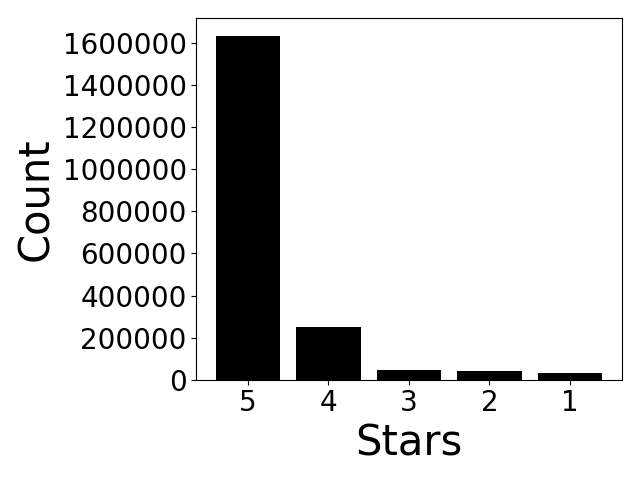
\includegraphics[width=0.45\linewidth]{arukereso}}
	\hspace{5pt}
	\subfigure[Legalább 10 hosszú]{
		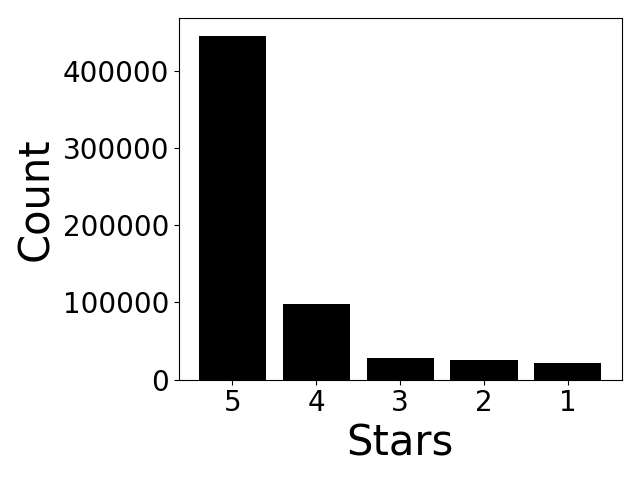
\includegraphics[width=0.45\linewidth]{arukereso10}}
	\caption{Vélemények eloszlása}
	\label{fig:arukereso}
\end{figure}

A leghosszabb vélemény 842 token-ből áll. A túl rövid értékelések kevés információval szolgálnak, így az eredeti adathalmazból a 10 token-nál rövidebb bejegyzéseket eltávolítottam.

Az így kapott adatsor átesett a szokásos előkészítési lépéseken. Ezen felül a 3 csillagos "semleges" véleményeket eltávolítottam, az 1-2 csillaggal rendelkező értékelések "negatív", a 4-5 csillaggal rendelkezők pedig "pozitív" címkét kaptak.

A halmazban a "pozitív" címkéjű vélemények szerepelnek túlnyomó többségben. A kiegyensúlyozatlansági probléma kivédésére több elemet töröltem a "pozitív" címkéjű elemek közül, így a két csoport egyenlő elemszámmal szerepel. Az előállított auto-annotált tanítóhalmaz 94982 adatponttal rendelkezik, mindegyik osztály 47491 méretű. 

Az \textit{arukereso}-nek elnevezett adathalmaz alkalmas lehet a szöveg érzelmi tartalma szerinti bináris klasszifikáció kivitelezésére. 
